

%% NOVAC
%% =============
%%
This chapter covers the algorithm which is used for the evaluation of the spectroscopic data recorded in NOVAC. 
The occurring problem of contamination of the reference is explained and possible solutions are presented.

\section{Conventional Evaluation Routine}
The fitting routine used for this thesis is based on the DOASIS software \cite{kraus2006doasis}. 
The equations of the DOAS retrieval of this work are slightly different from \Cref{eq:taustrich}.
\Cref{eq:lbe} can be rewritten as:
\begin{align}
ln\left(I\left(\lambda, L\right)\right) = &ln\left(I_0 \right) + P \left(\lambda\right) -	\int_{0}^{L}\sum_{j}\sigma_j \left(\lambda, p, T \right) \cdot c_j \left(l\right)dl \nonumber \\
= &ln\left(I_0 \right) + P \left(\lambda\right)-
\sum_{j}\sigma_j \left(\lambda, p, T \right) \cdot S_j
\label{eq:lben}
\end{align}
%
The term $ P \left(\lambda\right)$ is a polynomial that accounts for all broad-band effects which approximates the scattering effects of the atmosphere.

The remaining task of the DOAS routing is to find a model function $F \left(\lambda\right)$ that minimizes $\chi^2$:
\begin{equation}
\chi^2 = \sum_{i=\lambda_1}^{\lambda_2}\left(ln(I(i))-F(i)\right)^2
\end{equation}
While $F\left(\lambda\right)$ can be expressed on the basis of \Cref{eq:lben}:
\begin{equation}
F\left(\lambda\right) = ln\left(I_0 \right) + P \left(\lambda\right)-
\sum_{j}\sigma_j \left(\lambda\right) \cdot S_j
\label{eq:F}
\end{equation}
The DOAS fitting routine uses a combination of a standard least-squares fit and a Levenberg-Marquard algorithm to minimize $\chi^2$\\
\\
The \ce{SO2} evaluation takes place in the wavelength range between 314.8~nm and 328~nm. Including a \ce{SO2} absorption cross section recorded at a Temperature of 298K \cite{vandaele2009fourier} and a  \ce{O3} absorption cross section recorded at 221K \cite{burrows1999atmospheric}.\\
The \ce{BrO}  evaluation is performed for a wavelength range between 330.6~nm and 352.7~nm. The sum in \Cref{eq:F} includes for the BrO evaluation the following absorption cross sections:
\ce{BrO}  at 298K \cite{fleischmann2004new}, the \ce{SO2} and  \ce{O3} absorption cross sections described above and  \ce{O4} \cite{hermans2003absorption},  \ce{NO2} at 298K \cite{vandaele1998measurements} and  \ce{CH2O} at 298K \cite{meller2000temperature}.\\
%
The Network for Observation of Volcanic and Atmospheric Change provides spectral data for $\approx$ 50 different elevation angles. For the DOAS evaluation a reference and a measurement spectrum is needed. To get the SCD's the references need to be without any amount of the volcanic trace gas of interest (This will be discussed more detailed in \Cref{Chap:Cont}). With the $F\left(\lambda\right)$ the column density of  \ce{BrO}  and \ce{SO2} of the measurement spectrum relatively to the reference spectrum can be calculated using the calculations from above. \\
\\
\begin{figure}
	\subfigure[]{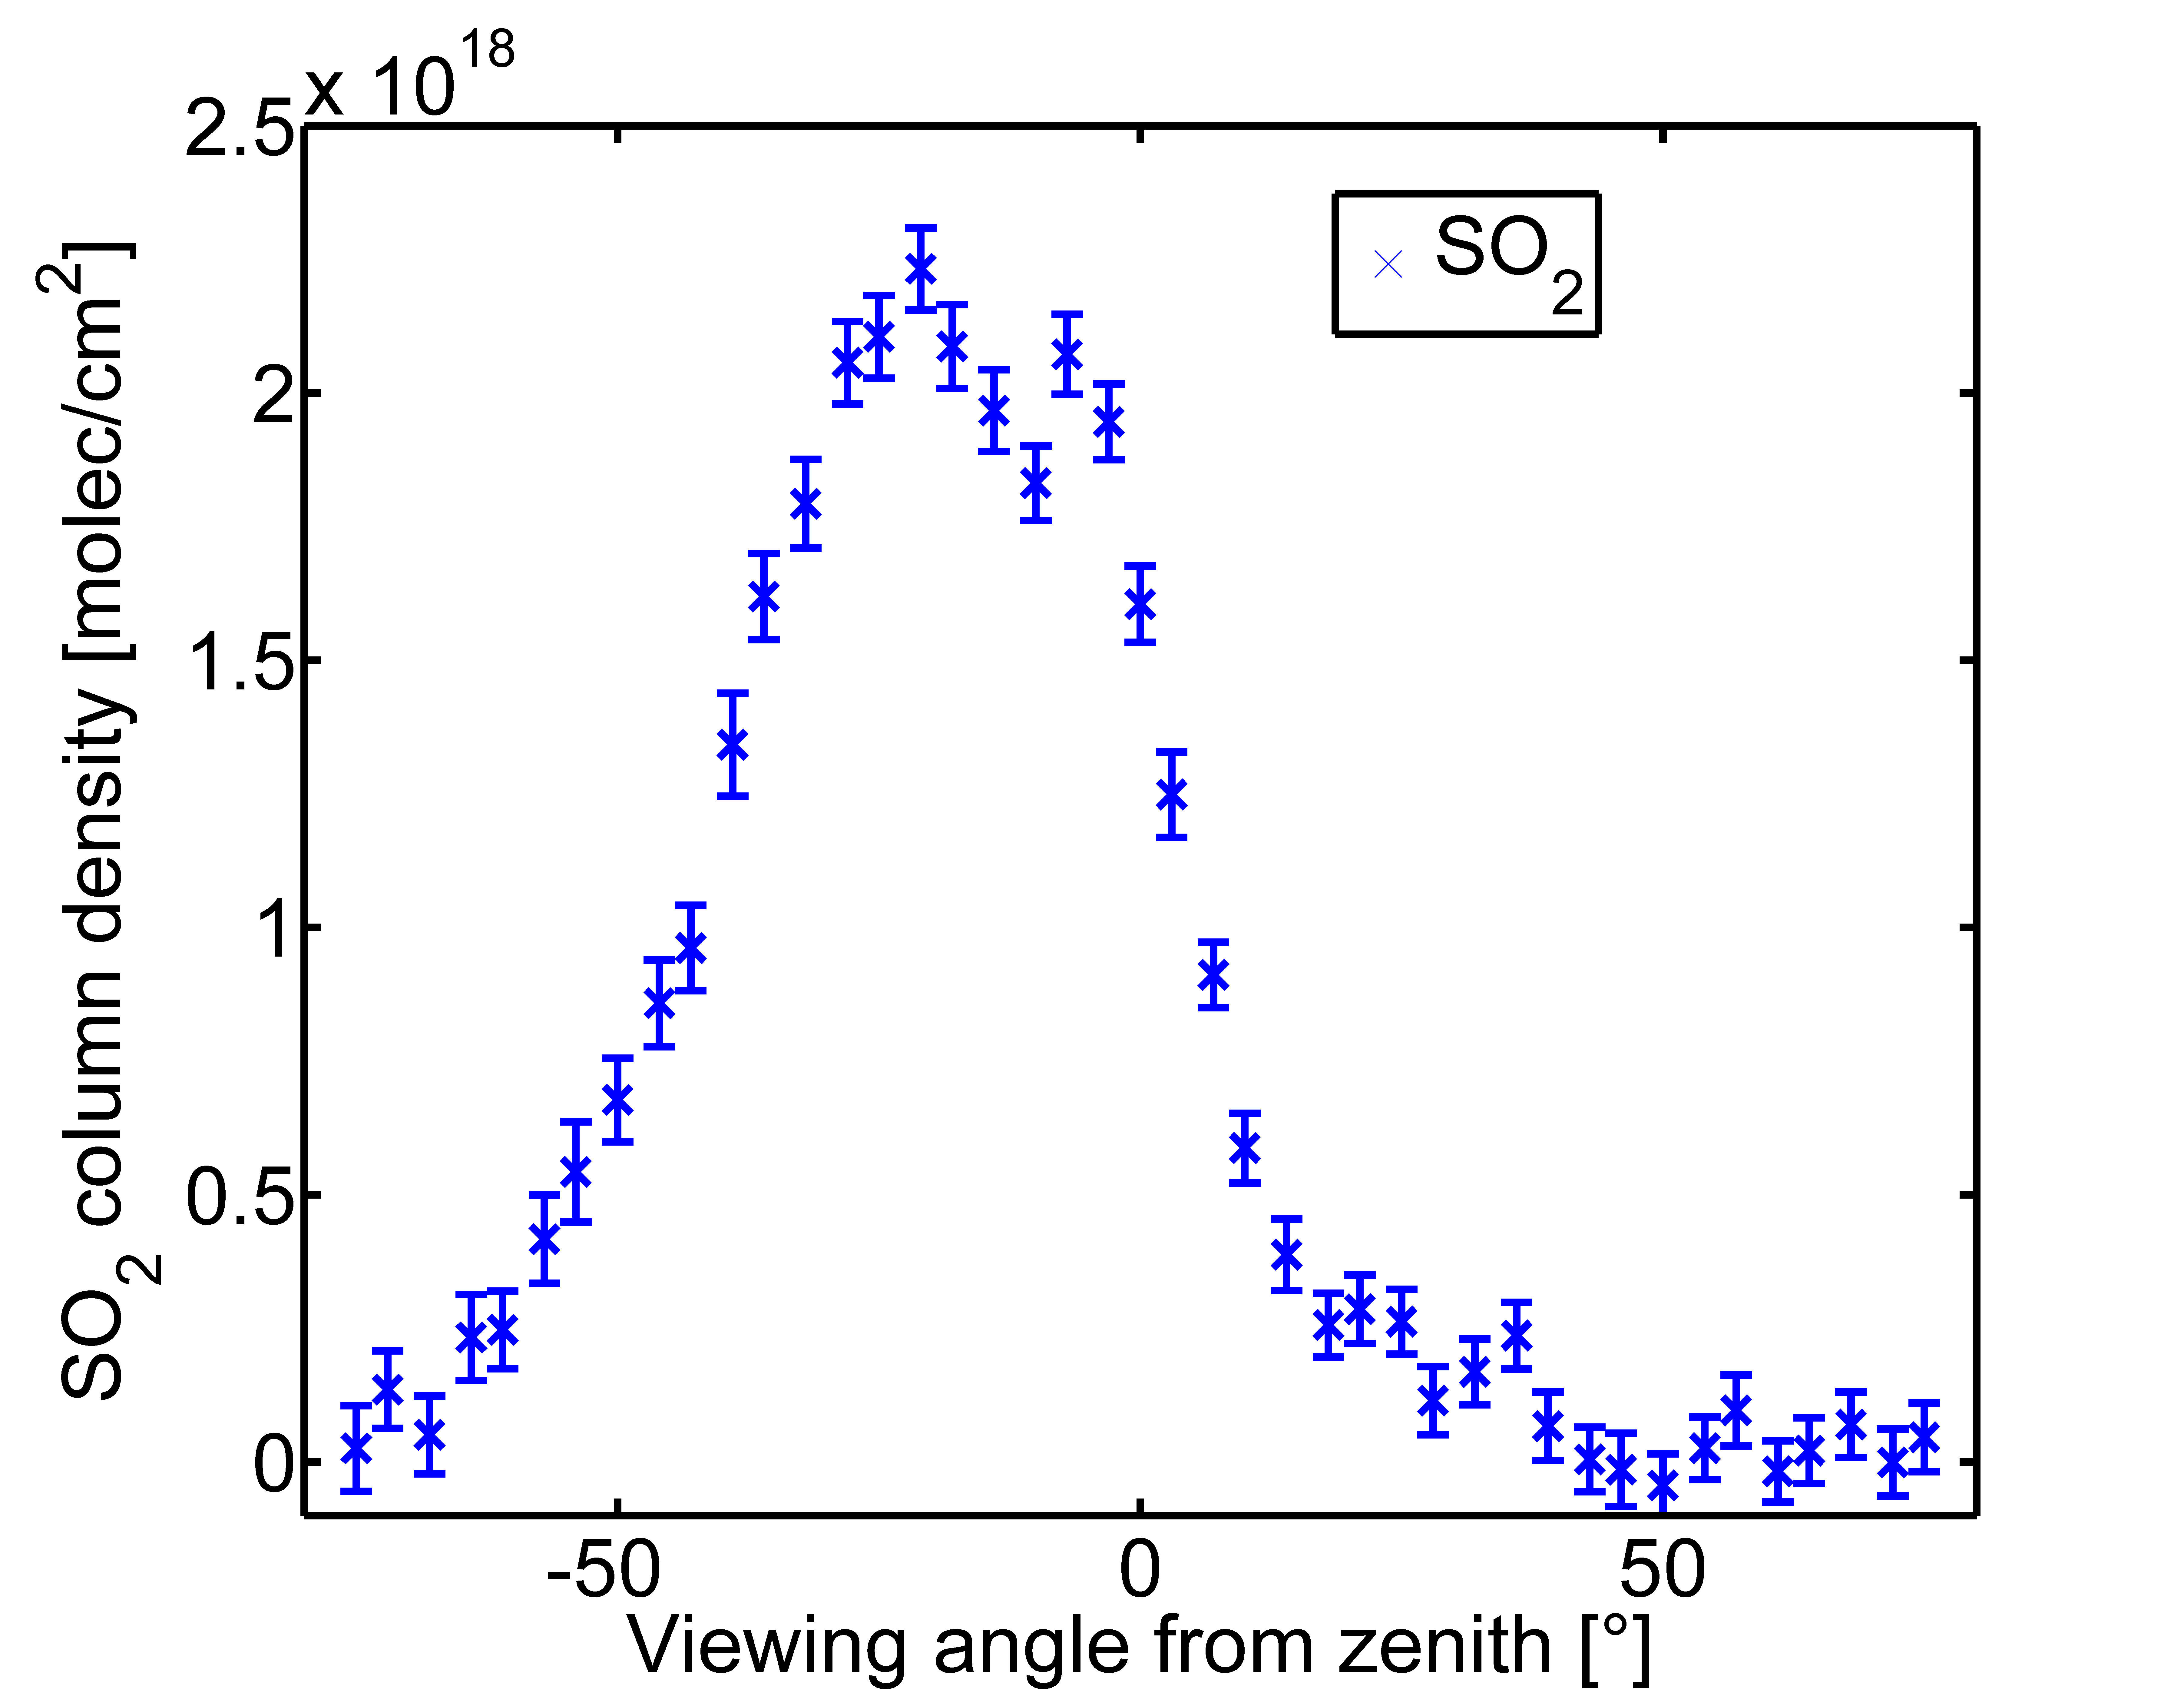
\includegraphics[width=0.51\textwidth]{Bilder/Simon/Bilder_Tung/SO2_Scan_0}}
	\subfigure[]{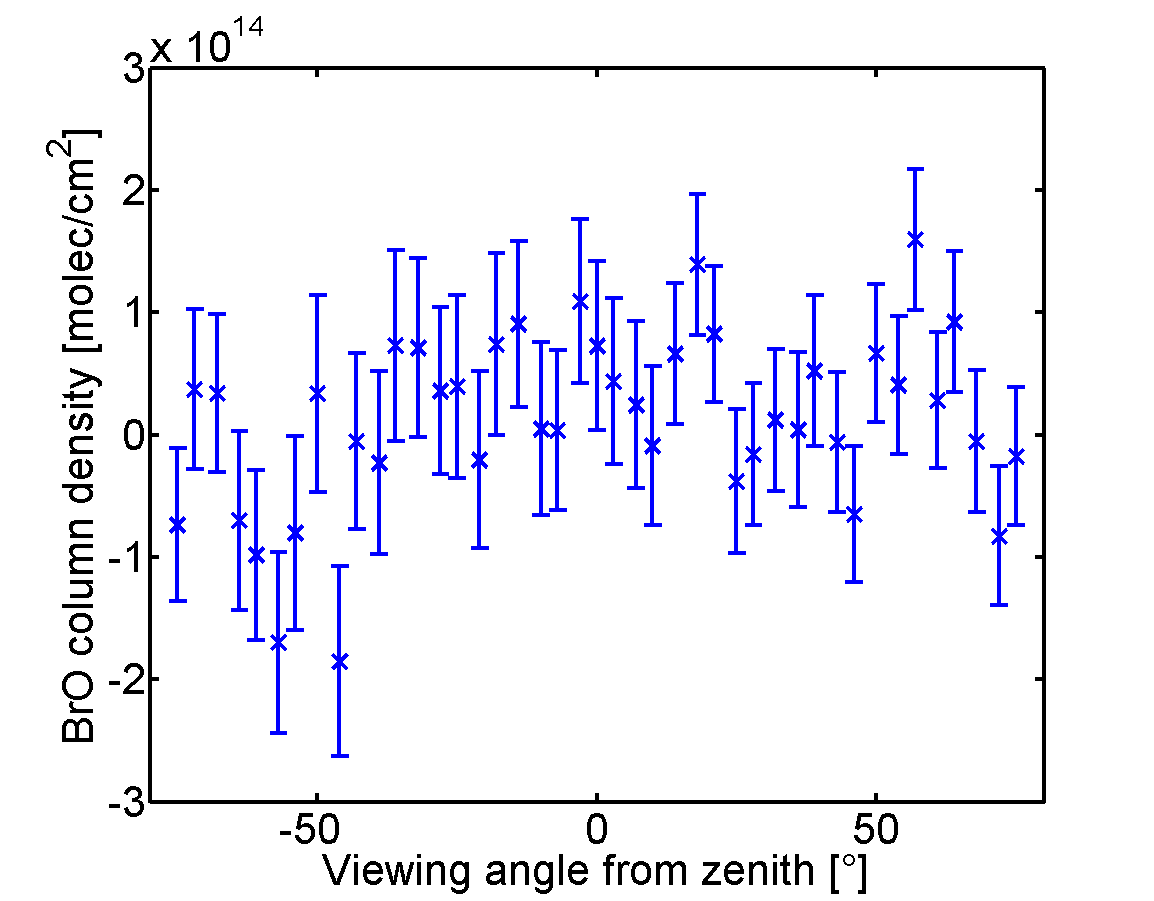
\includegraphics[width=0.51\textwidth]{Bilder/Simon/Bilder_Tung/BrO_Scan}}
	\caption{(a) \ce{SO2} SCD as a function of the elevation angle with error bars computed by the DOASIS fitting routin. (b) \ce{BrO} SCD as a function of the elevation angle with error bars computed by the DOASIS fitting routine.  Taken from \cite{WarnachSimon}}
	\label{fig:plumeref}
\end{figure}
%
In the following we describe the technical implementation of the DOAS approach using the data of NOVAC instruments:\\
\begin{figure}
	\centering
	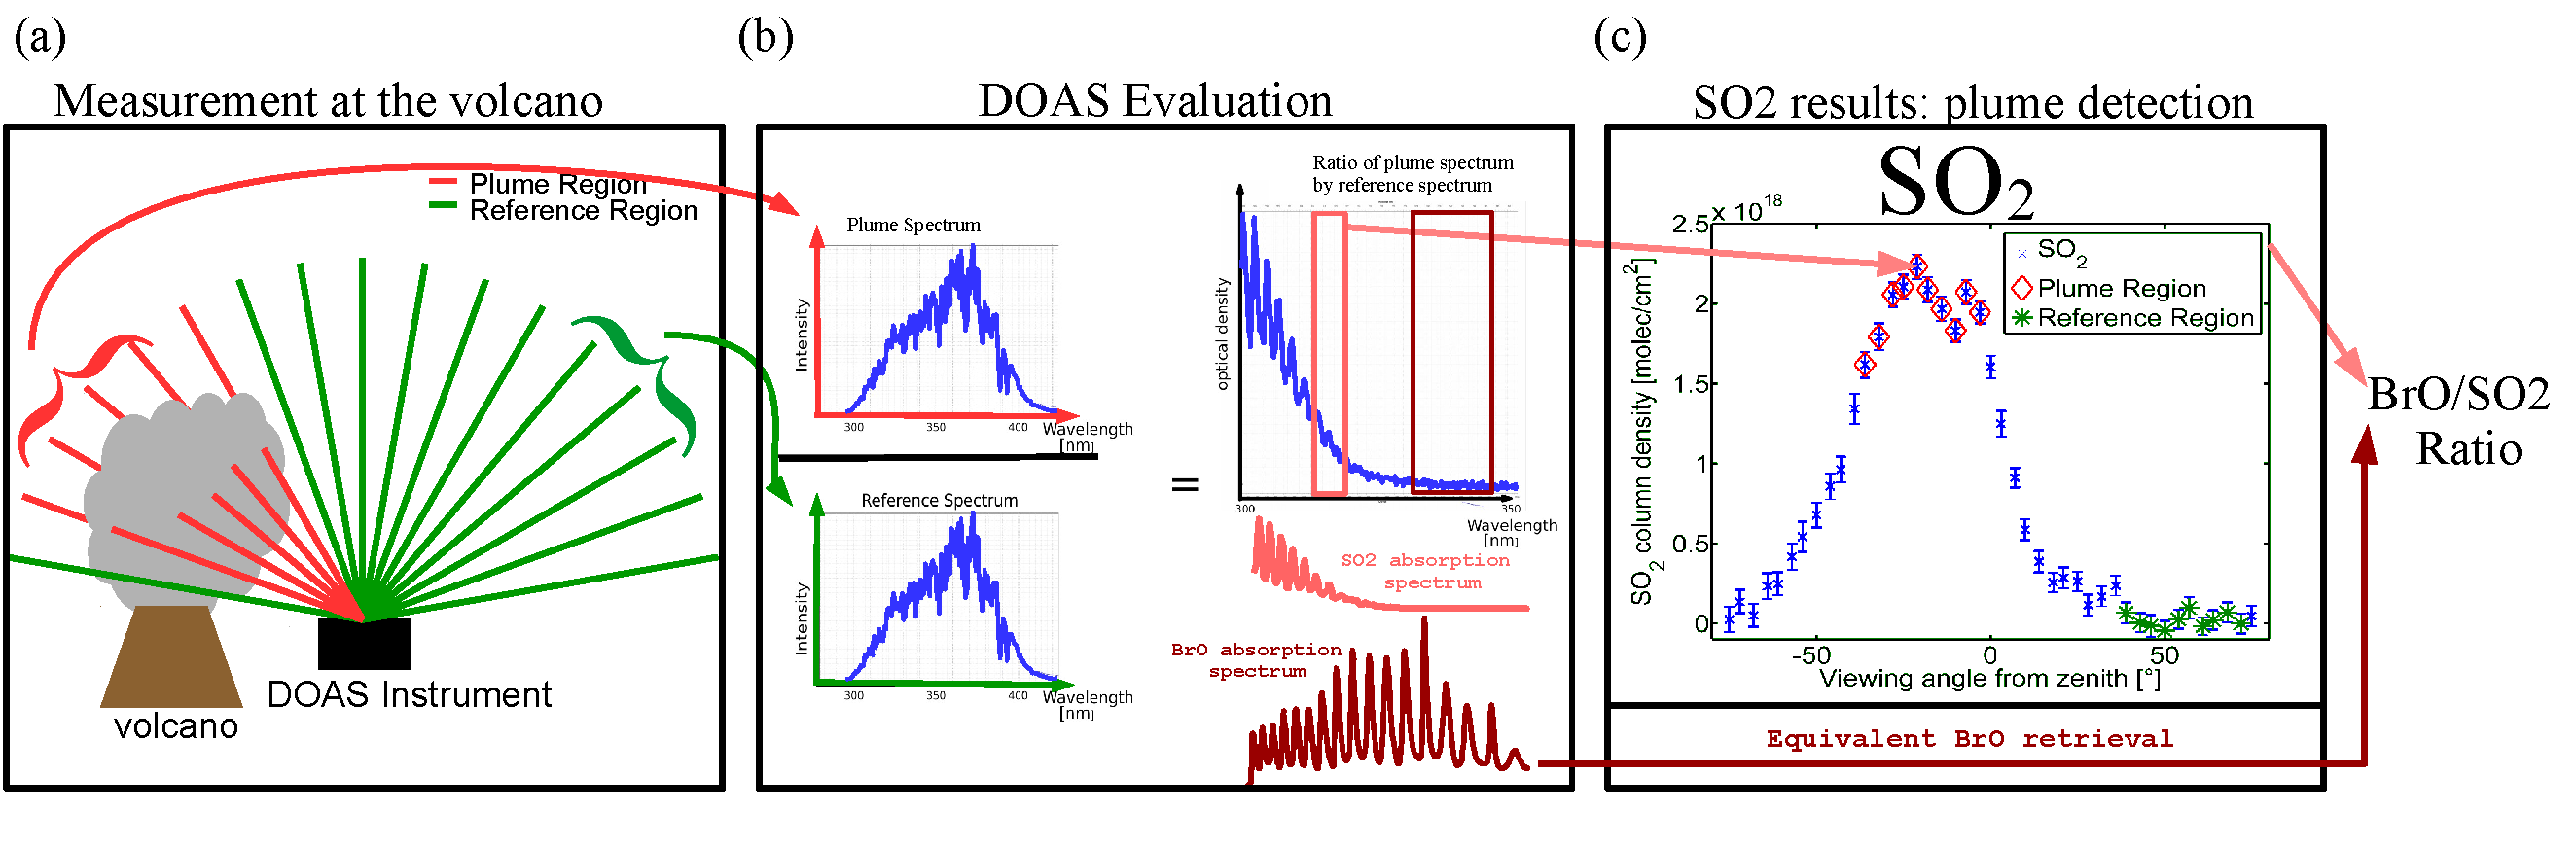
\includegraphics[width=1\linewidth]{Bilder/NOVAC_Eval}
	\caption{NOVAC Evaluation: (a) Measurement at the volcano (b) Evaluation of the spectral data with the DOAS routine using the absorption cross sections of \ce{BrO}  and \ce{SO2}. (c) finding the location of the plume and reference (d) the ratios BrO/\ce{SO2} at Tungurahua. }
	\label{fig:NOVAC_Eval}
\end{figure}
%
The first step is to correct each spectra of the scan for dark current and offset using the dark current spectrum.
The next important task is to locate the measurement spectrum and the reference region in the volcano plume. 
To do so, the pre-reference (the spectrum recorded at an elevation angle of  0$^{\circ} $) is used to perform the evaluation of the scan spectra recorded at every elevation angle.
For every spectrum of the scan the \ce{SO2} differential slant column density (dSCD) with respect to the pre-reference is calculated using \Cref{eq:F} by the DOASIS fit routine.

The result is \ce{\ce{SO2}} dSCDs as a function of the elevation angle. So we can localize the maximum and the minimum of \ce{\ce{SO2}}
The location of the \ce{\ce{SO2}} maximum defines the location of the plume. We assume that the minimum of the \ce{\ce{SO2}} curve corresponds to a region outside of the plume which is true in most times. The \ce{\ce{SO2}} amount in the earths atmosphere is negligible (see  \Cref{chap:so2}) so we take it as a region of zero \ce{SO2}. \\
To technically detect the plume region we use a gauss fit of the \ce{SO2}-elevaltion-angle-curve.
To increase the quality and to get a more robust result the sum over several plume spectra is taken. If the gauss curve is too wide we use only the 10 spectra with the highest \ce{SO2} amount. For the reference we use the sum of the 10 spectra with the lowest \ce{SO2} amount.\\
%
%	\begin{figure}
%		\centering
%		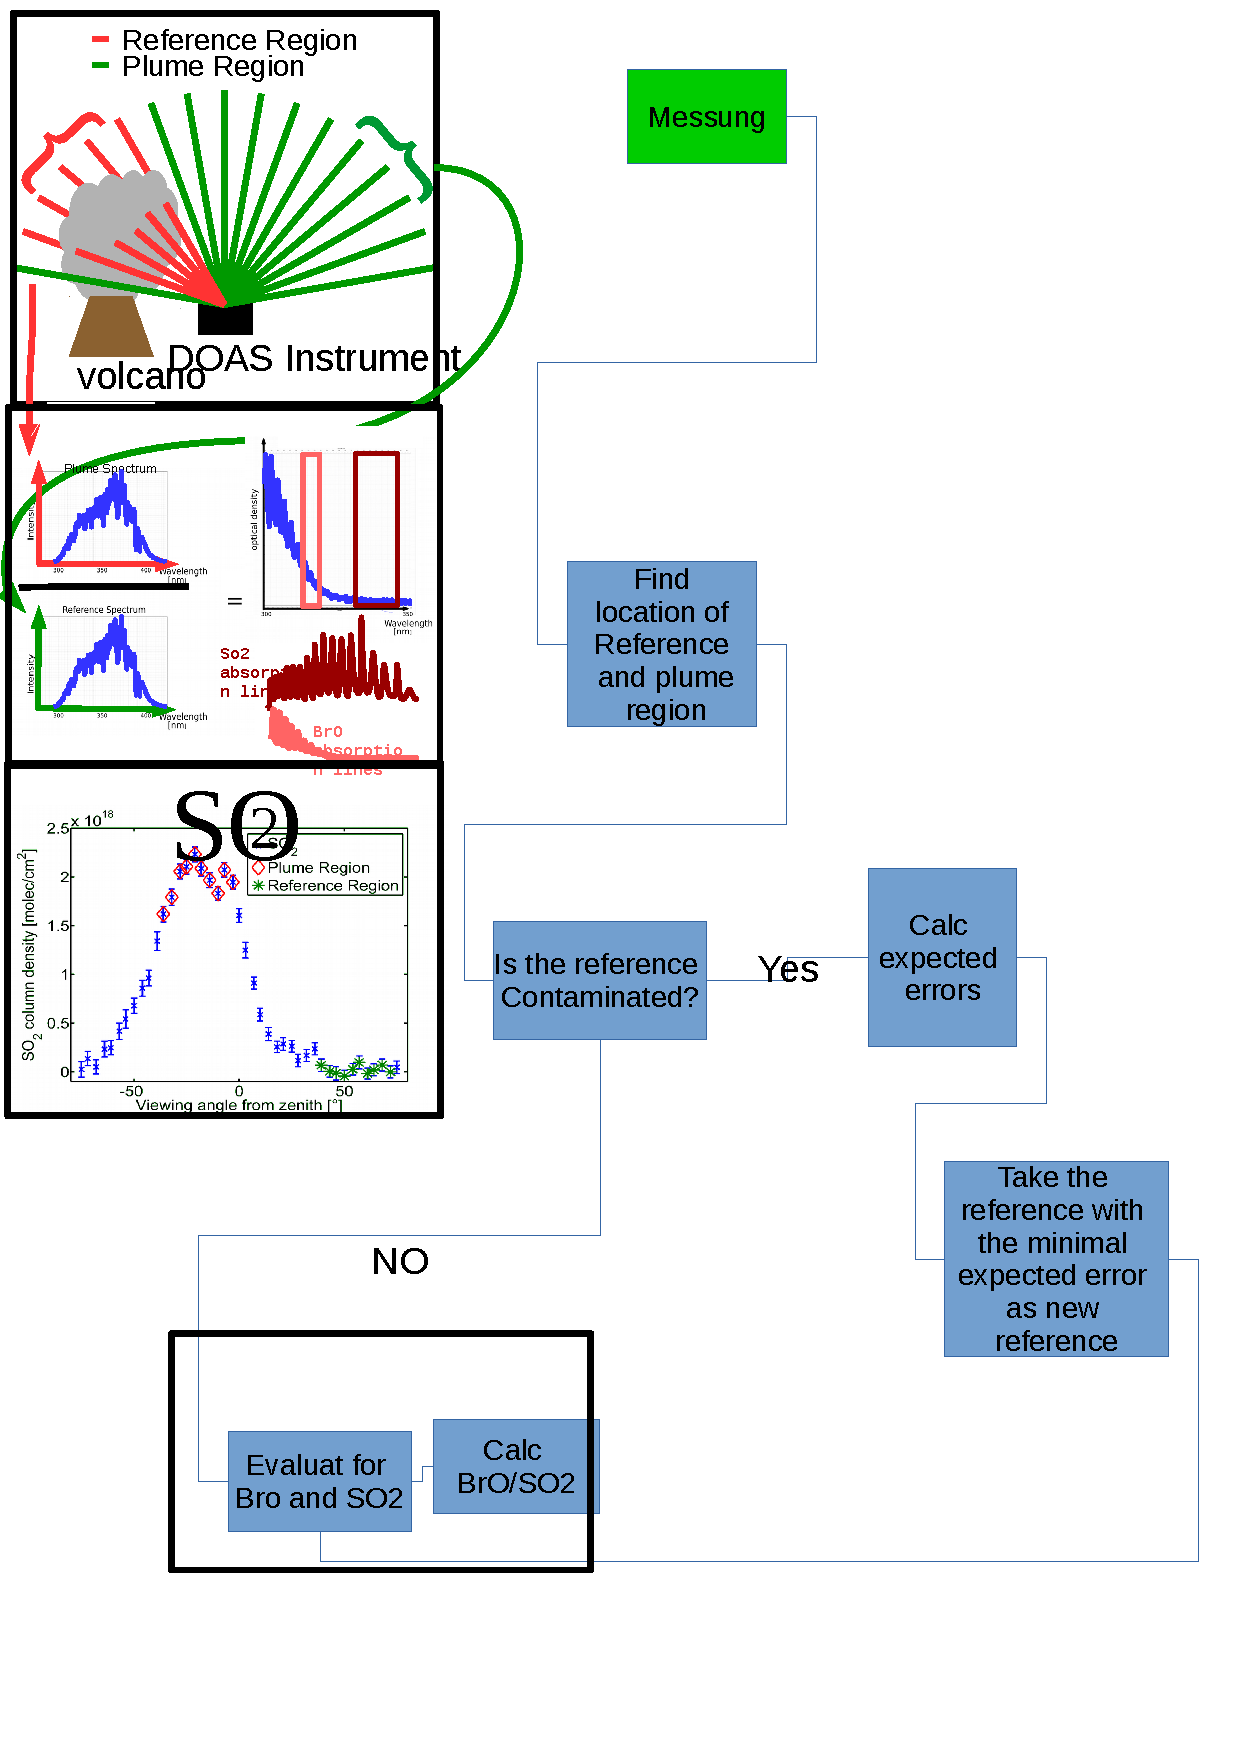
\includegraphics[width=0.7\linewidth]{Bilder/DOAS_Routine}
%		\caption{Sketch of the DOAS Routine }
%		\label{fig:FlussDiag}
%	\end{figure}
The absolut slant column densities (SCD's) of \ce{BrO}  and \ce{SO2} can now be calculated with the so found reference and plume spectrum.
In \Cref{fig:plumeref} (a) an example \ce{SO2} SCD as a function of the elevation angle is shown. The \ce{SO2} curve has a maximum at the position of the plume at an elevation angle of approximately $-30^{\circ}$ to $0^{\circ}$  and a reference region at an elevation angle of $40^{\circ}$ to $70^{\circ}$. \Cref{fig:plumeref} (b): The extrema of the \ce{BrO}  curve are not as distinct as it is the case for the \ce{SO2} curve.
Since the \ce{BrO} column density is much lower than the \ce{SO2} column density, and just lies slightly above the detection limit, the plume is hard to detect using the \ce{BrO} column density as it is shown in fig. \ref{fig:plumeref} (b). 
Therefore we use plume location we found by using \ce{SO2} to evaluate the \ce{BrO} column density.\\
To further increase the fit quality multiple reference and plume spectra of successive measurements are added.
\Cref{fig:algorithm} (b) shows the routine of adding multiple spectra of consecutive measuring times. In the following those spectra which result of multi adding technique will be named "Multi Add Spectra".\\
%
Taking the \ce{BrO}/\ce{SO2} ratio if the column densities are close to zero yields unpredictable and unrealistic results. Thus, spectra measured outside of the volcano plume need to be excluded.
This could be achieved by setting a \ce{BrO} or/and an \ce{SO2} threshold. A reasonable \ce{BrO} threshold need to be at least in the order of the DOAS fit error. However this could lead to elevated \ce{BrO}/\ce{SO2} ratios, since the \ce{BrO} error is often close to the detection limit. Thus, all low \ce{BrO} column densities are excluded from the evaluation.
%
\begin{figure}
	\subfigure[ ]{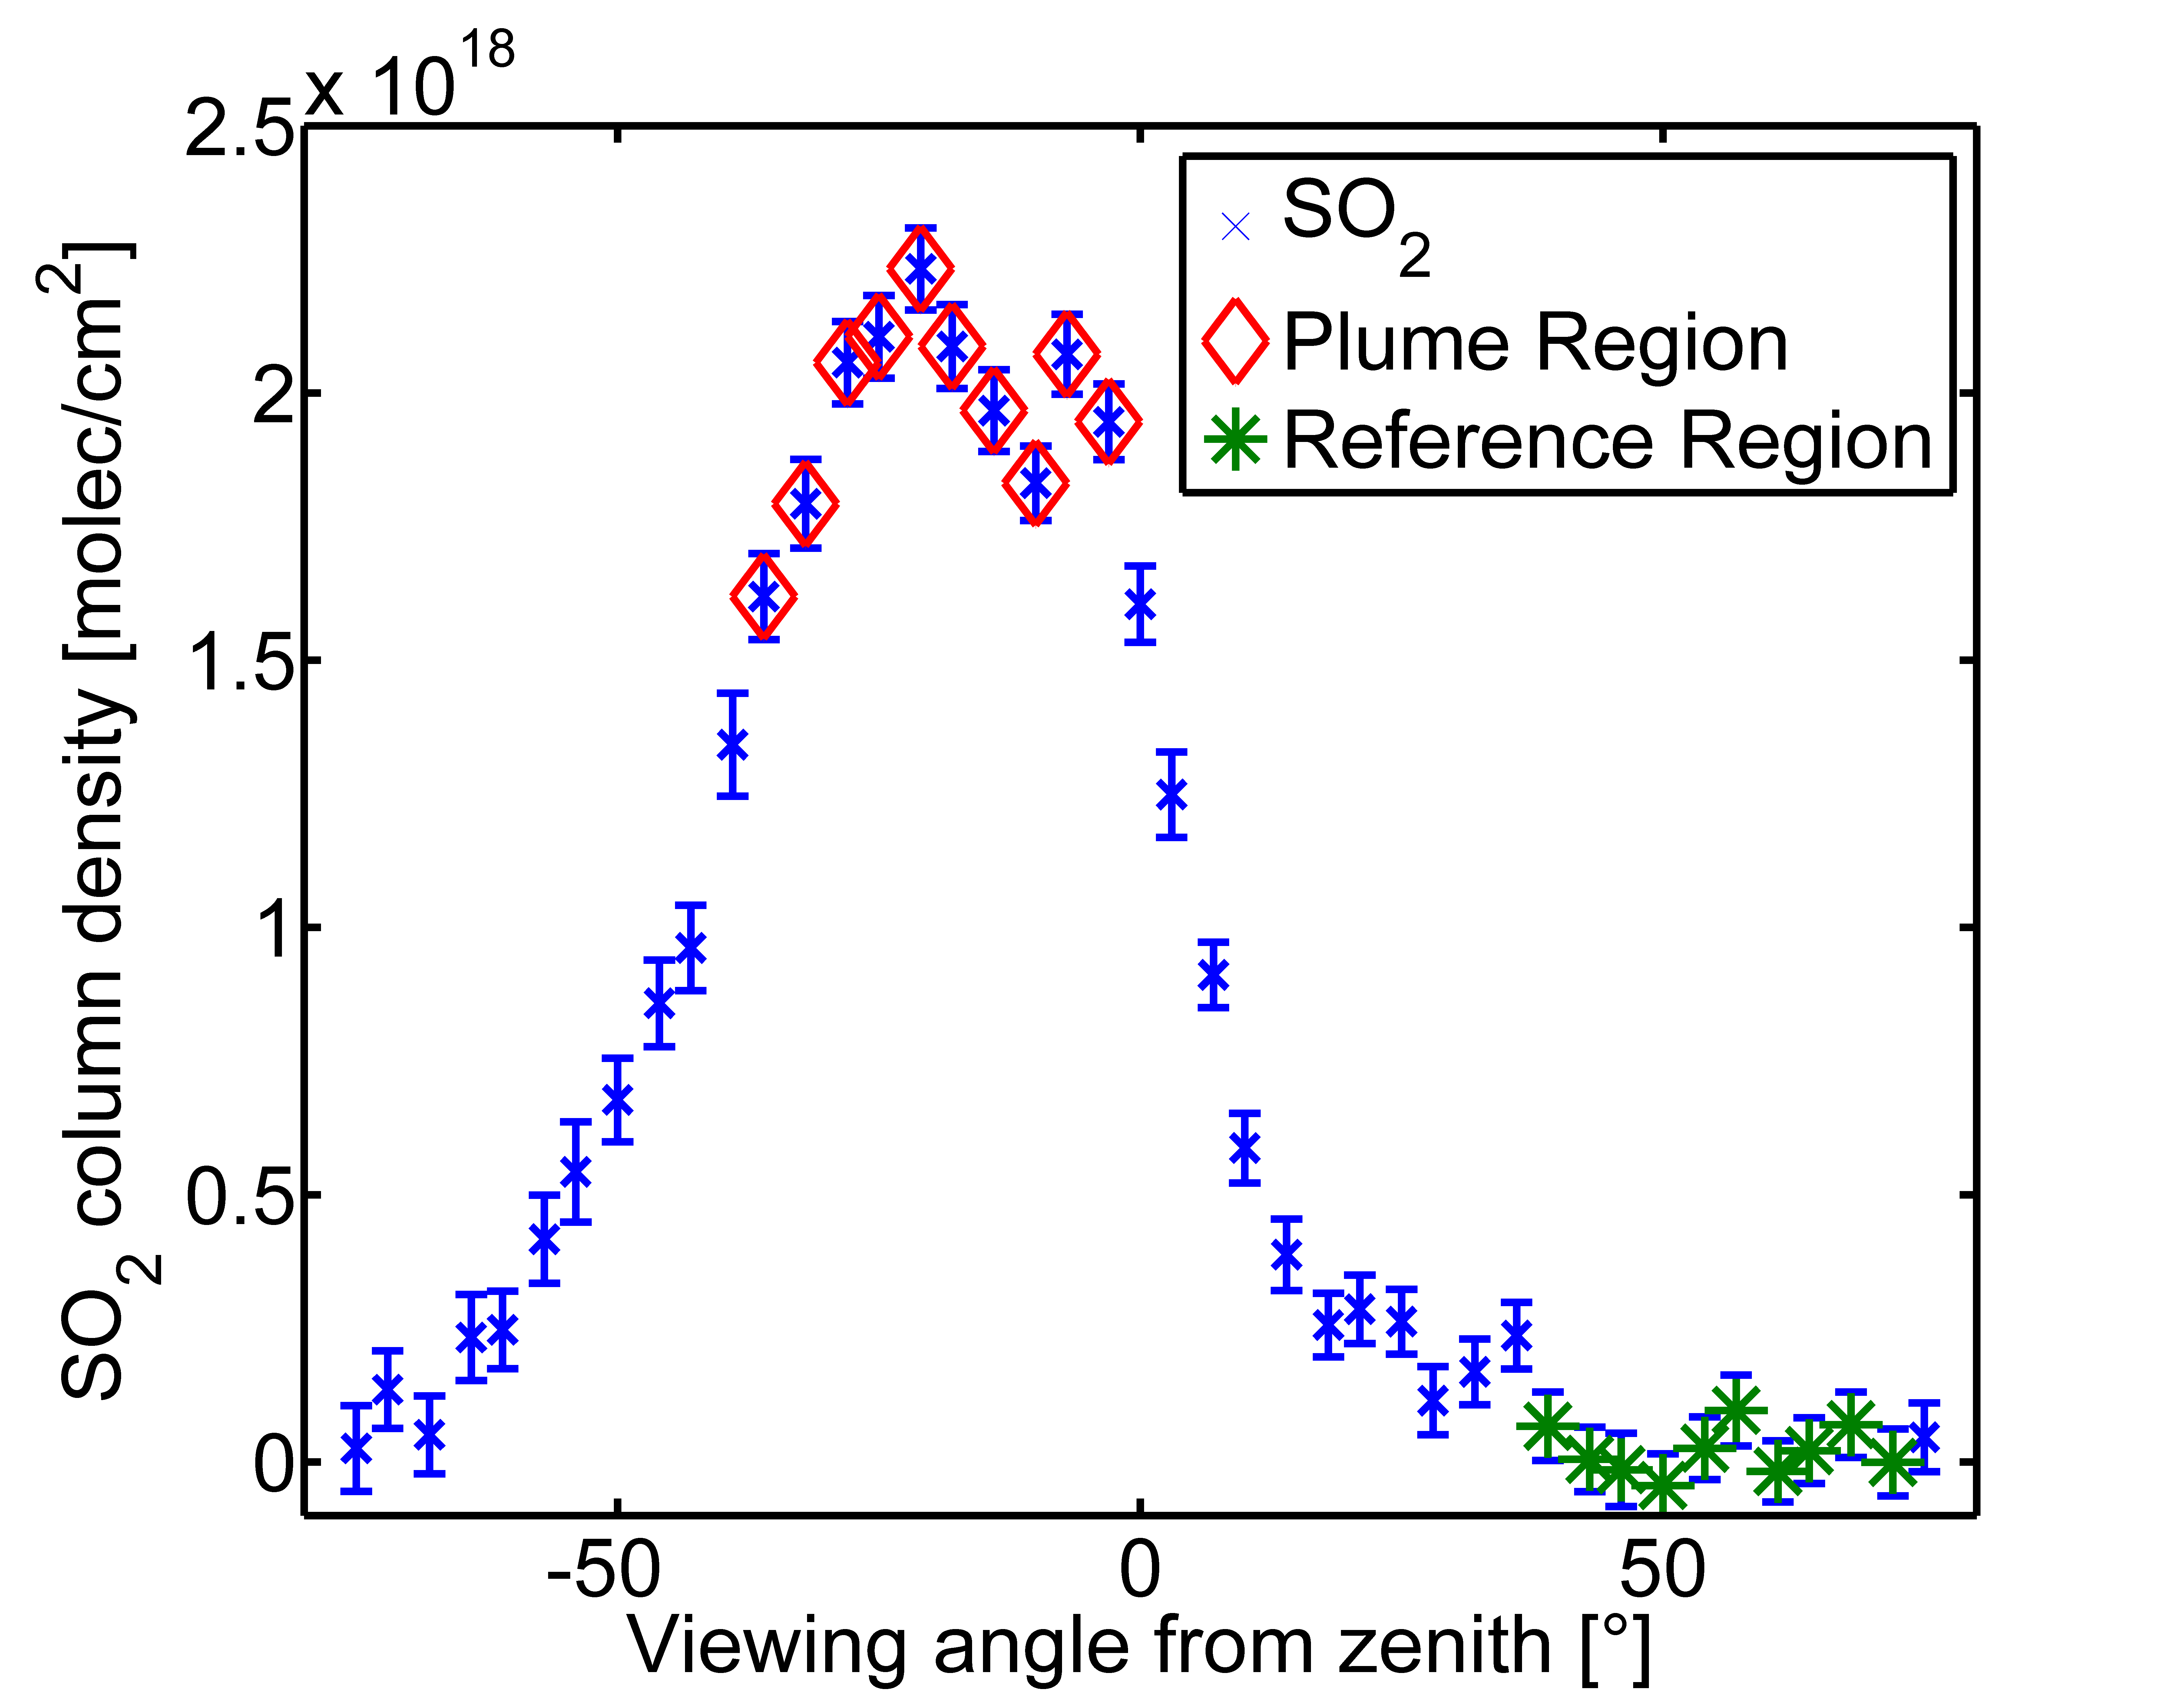
\includegraphics[width=0.53\textwidth]{Bilder/Simon/Bilder_Tung/SO2_Scan}}
	\subfigure[ ]{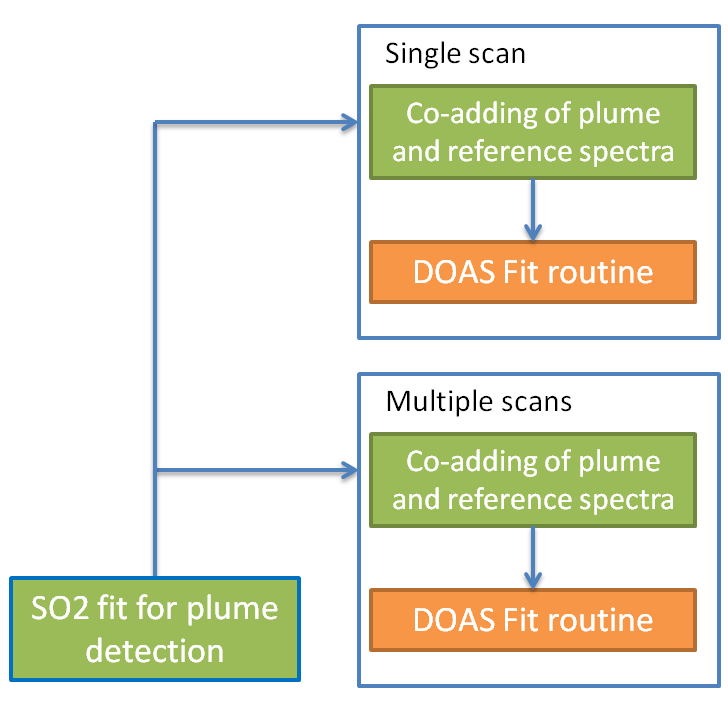
\includegraphics[width=0.47\textwidth]{Bilder/Simon/Bilder_Tung/Algorithm}}
	\caption{(a) \ce{SO2} SCD as a function of the elevation angle. The co-added plume region is marked with red diamonds, and the co added reference region with green stars. From \cite{WarnachSimon}. (b) Flow chart of the \ce{BrO}  and \ce{SO2} evaluation. From \cite{lubcke2014optical}.}
	\label{fig:algorithm}
\end{figure}
The other possibility is to set a \ce{SO2} threshold. In this thesis an \ce{SO2} threshold (plume limit) of $7\cdot 10^{17} \frac{molec}{cm^2}$ is used for the selection of spectra for the evaluation of the \ce{BrO}/\ce{SO2} ratio. $7\cdot 10^{17} \frac{molec}{cm^2}$ is a relatively high column density. However, this this approach assures that no significant amount of gases will be filtered out, therefore the BrO/\ce{SO2} ratio will not be significantly influenced \citep{lubcke2014bro} and that all utilized measurement spectra will be inside of the volcano plume. \\
Setting a plume limit leads to an decrease of usable data. The share of usable  data as a function of the plume limit is shown in \cref{fig:percentageminso2}. An exponential decrease of data can be observed. The plot is based on the data of Tungurahua. Plume limits below 7$\cdot10^{17}$ are shaded with yellow. A plume limit of 7$\cdot10^{17}$leads to a data share of approximately 10\%.
\begin{figure}
	\centering
	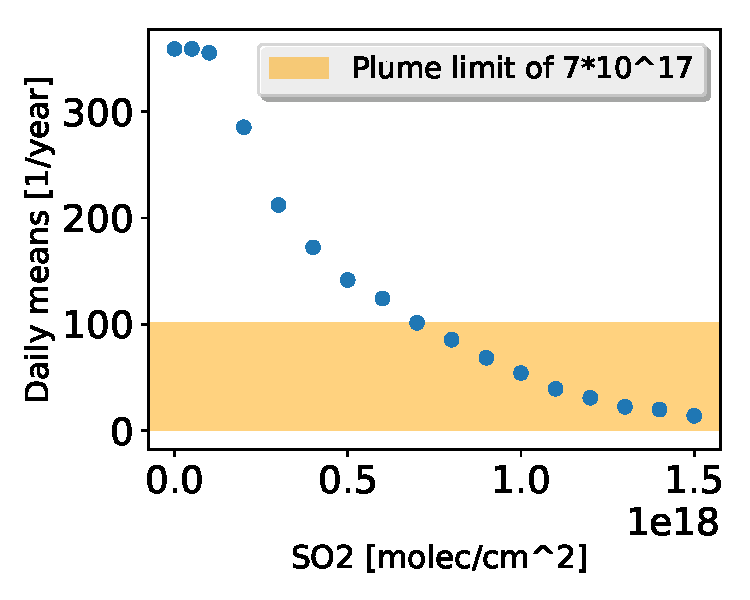
\includegraphics[width=0.7\linewidth]{Bilder/percentage_minSO2}
	\caption{The decrease of the amount of usable data as a function of the plume limit. The plume limits below the actual plume limit of 7$\cdot10^{17}$ are marked with a yellow shade.}
	\label{fig:percentageminso2}
\end{figure}

\section{Contamination Problem\label{Chap:Cont}}
To assure that the reference is volcanic gas free a high resolution solar atlas spectrum (see \Cref{kuruz}) was used to evaluate the reference. In some reference spectra an amount of \ce{SO2}  differeng from zero was found. Thus we can conclude, that there are some references which contains a not negligible amount of volcanic trace gases.
In rare (ca. 10\% of the data) scenarios, the
volcanic plume covers the whole scan region.
This could happen if for example the volcanic plume of the day before still extend over the hole scan area as a consequence of windless conditions.
In consequence, the reference	is contaminated with volcanic trace gases. Thus, the gas amount is underestimated by the NOVAC-Evaluation: In \Cref{fig:contaminated} we see an example from April 2011 (Tungurahua) where the reference region is contaminated by volcanic trace gases. The blue \ce{SO2} curve shows the calculations with the NOVAC-evaluation, but since there is still \ce{SO2} in the reference region, the assumption, that the \ce{SO2} amount could be set to zero in the reference region is wrong. The red curve shows the real \ce{SO2} curve, which lies significantly above the NOVAC -curve.\\
\\	
%
\\
\begin{figure}
	\centering
	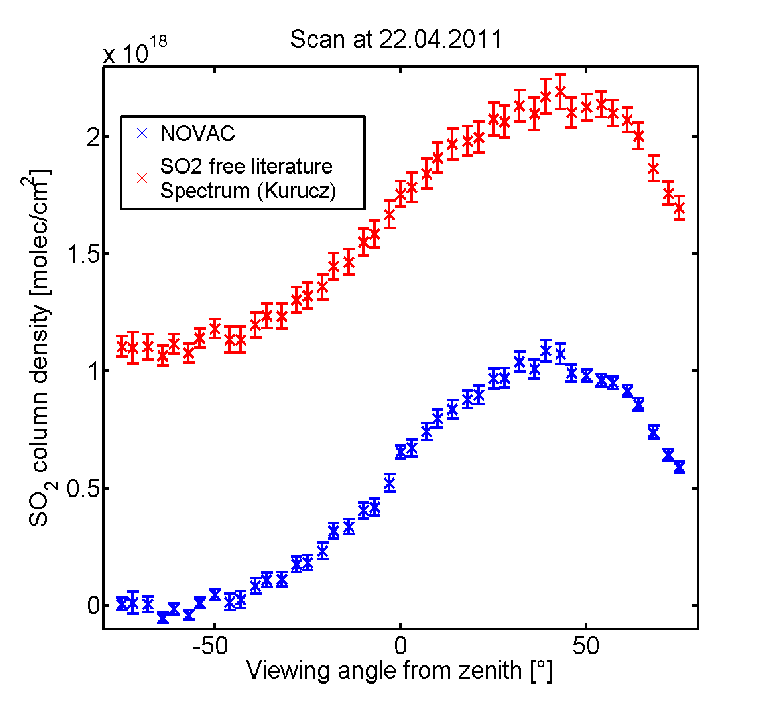
\includegraphics[width=0.7\linewidth]{Bilder/contaminated}
	\caption{Scan with a contaminated reference spectrum from April 2011. From \cite{WarnachSimon}}
	\label{fig:contaminated}
\end{figure}
If the reference region is for any reason
contaminated by volcanic trace gases, there are two possibilities: excluding the contaminated data from the evaluation or the reference spectrum has to be
replaced by a volcanic-gas-free reference. Alternative spectra are a
theoretical solar atlas spectrum or a volcanic-gas-free reference
spectrum recorded by the same instrument.\\ 
%
\\
%
In the following we will discuss both of the alternative reference spectra.
%
\subsection*{Evaluation using a Solar Atlas Spectrum \label{kuruz}}
An alternative for choosing the region with the lowest column density as reference region is to use a theoretical high resolution solar atlas spectrum as reference \cite{chance2010improved}.
The use of a theoretical solar atlas spectrum as a reference which is completely volcanic-trace-gases-free was first proposed by \cite{lubcke2014bro}.
The advantage of using a solar atlas spectrum as reference is, that we know that there are no volcanic trace gases. Thus, we know that the reference is free of volcanic trace gases and do not need to take this fact as a possibly inadmissible assumption. The disadvantage is, that using a solar atlas spectrum comes along with a drawback of precision: A theoretical solar atlas spectrum is far more precise than the spectra of the NOVAC instruments. Therefore the instrument functions need to be modeled and added to the retrieval.\\ 
The reduction of precision is acceptable for the
\ce{SO2} retrieval but not suitable for a \ce{BrO} retrieval because then most data would be below the detection limit.\\
%
\\
%
Possible contaminations can be checked
by a theoretical solar atlas spectrum to evaluate the \ce{SO2} amount in the reference.
%
\subsection*{Evaluation using a Spectrum of the same Instrument}
An alternative reference spectrum could be a volcanic-gas-free reference
spectrum recorded by the same instrument at a different time. When using such a reference several problems occur:\\
As described in \Cref{NOVAC} the instruments used in NOVAC do not include features like temperature stabilization. Due to that the measurements are not independent from external parameters. 
So we need to choose a reference recorded at similar conditions with respect to meteorology and	radiation as well as in the temporal proximity due to instrumental changes with time and ambient conditions. Ideally the external conditions should be equal to the conditions when the plume was recorded.\\
\\
%
\\
In this work we combine both options in order to
achieve both, enhanced accuracy but still maximum possible precision of
the \ce{SO2} and \ce{BrO} retrievals. So we use the solar atlas spectrum to check for 
contamination and a reference spectrum recorded in temporal proximity by the same instrument as reference.\\
\\
Thus if contamination occurs it is possible to choose from a list of gas free alternative references. In theory, for ideal instruments a references should lead to the same results for the gas retrievals. But instruments are imperfect (see \Cref{NOVAC}) thus the reference need to be chosen carefully an order to improve the results.\\
%
\\
As discussed above it might occur, that, that the reference is contaminated for example by the plume of the day before. If that happens, we underestimate the gas amount by using a contaminated reference. But another possibility is, that the plume is also contaminated. This might be the case if the volcanic gas of the volcano is not taken away by the wind, but accumulates at the instrument. If this is the case, using an other reference would lead to an overestimation of the column density of gases. With the data retrieved by the NOVAC instruments it is very difficult up to impossible to discover whether the plume is contaminated or not. \\
\Cref{fig:contaminationdependencyso2} shows the strength of contamination as function of the mean SO2 amount of the day before. The strength of contamination is  measured as the difference when perform the evaluation for SO2 with the contaminated reference recorded as the same time as the plume spectrum was recorded and when using a gas free reference. The data where fitted with a linear function. The left plot shows data from the Tungurahua volcano, right the data of Nevado Del Ruiz are visualized. Even though both plots show a slightly increase of contamination strength with the mean amount of SO2 of the day before, the increase is not significant.\\
\\
However this thesis is build on the assumption, that the plume is free of additional contamination. In the following we discuss how to find the an optimal reference from another scan automatically.
\begin{figure}
	\subfigure{
	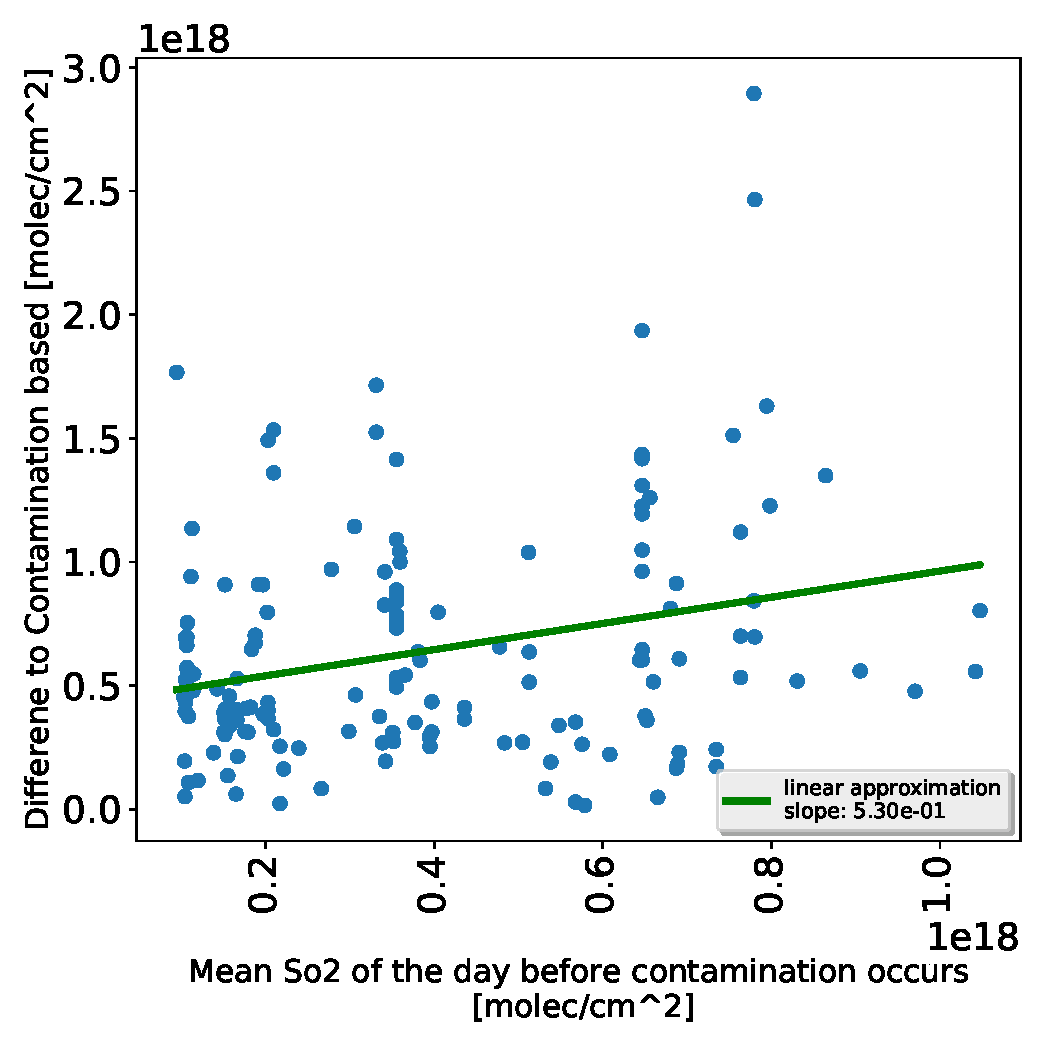
\includegraphics[width=0.5\linewidth]{Bilder/contaminationdependency_so2}}
\subfigure{
	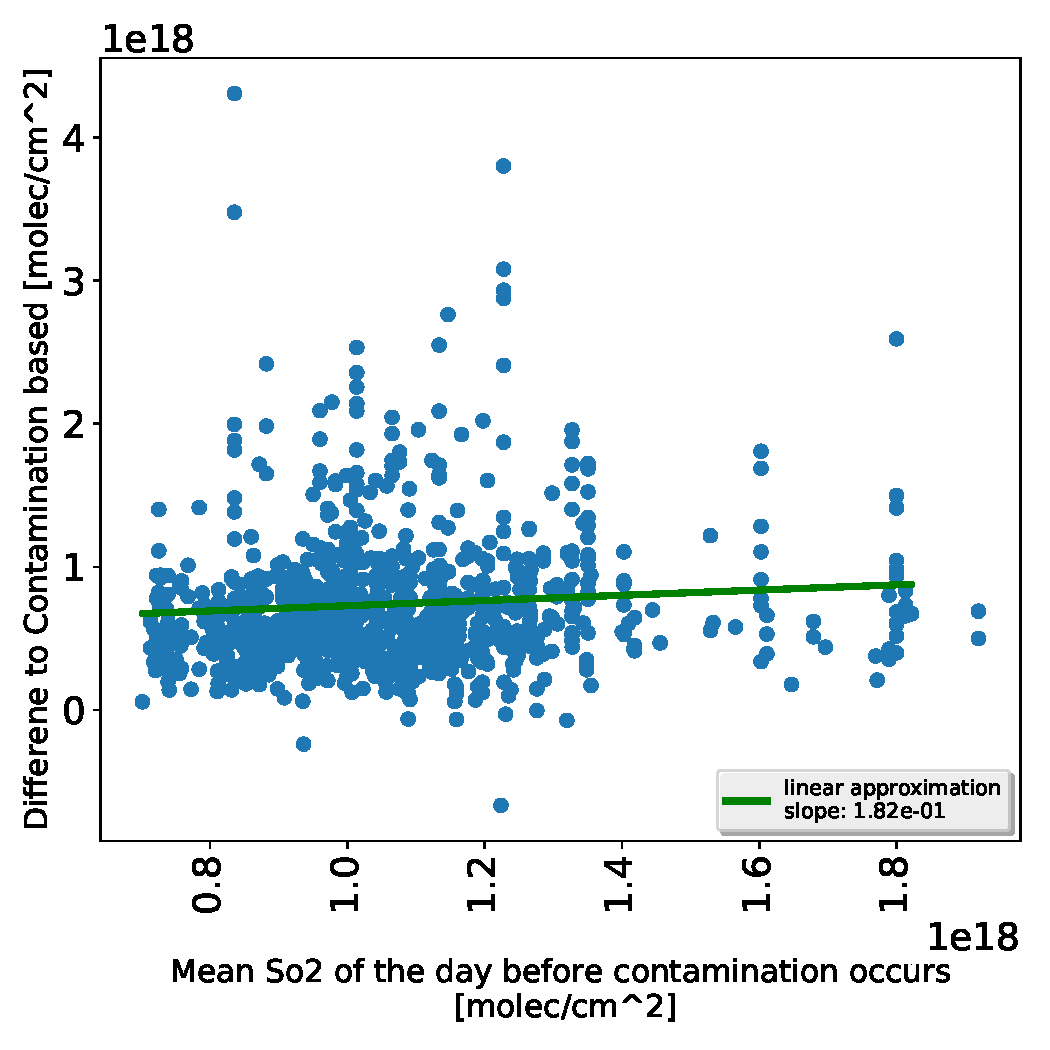
\includegraphics[width=0.5\linewidth]{Bilder/contaminationdependency_so2_Nevad}}
	\caption{The strength of contamination as function of the mean SO2 amount of the day before, The strength of contamination is defined as the difference in SO2 SCD  when evaluation with an alternative reference, or neglect the contamination. Left: data from Tungurahua. Right: Data from Nevado Del Ruiz. }
	\label{fig:contaminationdependencyso2}
\end{figure}